\documentclass[12pt,a4paper]{article}
\usepackage[polish]{babel}
\usepackage[T1]{fontenc}
\usepackage{lmodern}
\usepackage[utf8x]{inputenc}
\usepackage{hyperref}
\usepackage{url}
\usepackage{graphicx}
\usepackage{listings}
%\usepackage{xcolor}
\usepackage{color}
\usepackage{float}
\usepackage{multicol}
\usepackage{tikz-er2}
\usetikzlibrary{er,positioning,shadows}
\usepackage{makecell}
\renewcommand{\arraystretch}{1.5}

% TIKZ 
\tikzstyle{every entity} = [top color=white, bottom color=blue!30, 
                            draw=blue!50!black!100, drop shadow]
\tikzstyle{every weak entity} = [drop shadow={shadow xshift=.7ex, 
                                 shadow yshift=-.7ex}]
\tikzstyle{every attribute} = [top color=white, bottom color=yellow!20, 
                               draw=yellow, node distance=1cm, drop shadow]
\tikzstyle{every relationship} = [top color=white, bottom color=red!20, 
                                  draw=red!50!black!100, drop shadow]
\tikzstyle{every isa} = [top color=white, bottom color=green!20, 
                         draw=green!50!black!100, drop shadow]

% SETTINGS
\addtolength{\hoffset}{-1.5cm}
\addtolength{\marginparwidth}{-1.5cm}
\addtolength{\textwidth}{3cm}
\addtolength{\voffset}{-1cm}
\addtolength{\textheight}{2.5cm}
\setlength{\topmargin}{0cm}
\setlength{\headheight}{0cm}
% GO GO GO
\title{Academic Data Deliverer\\Bazy Danych}
\author{Artur Bednarczyk, Dawid Grajewski, Damian Kwaśniok\\Politechnika Śląska\\Wydział Matematyki Stosowanej\\Informatyka, semestr IV}
\date{\today}

\begin{document}
	\maketitle
	\begin{figure}[H]
		\centering
		\includegraphics[width=0.5\linewidth]{LOGO2}
		\label{fig:logo}
	\end{figure}
	\clearpage
	\tableofcontents
	\clearpage
	\section{Opis projektu}
		\subsection{Opis}
			Aplikacja dla studentów umożliwiająca łatwą i szybką wymianę notatek.
		\subsection{Funkcjonalności}
			\subsubsection{Logowanie i Rejestracja}
				Zaloguj się gdziekolwiek jesteś.
			\subsubsection{Przypasanie do grup}
				Zapisz się do grupy Twojej uczelni/wydziału/kierunku.
			\subsubsection{Notatki}
				Oglądaj i dodawaj nowe notatki.
	\section{Rozwiązania}
		\subsubsection{Technologie}
			.NET, C\#, MySQL.
		\subsubsection{Oprogramowanie}
			Visual Studio 2015
	\section{Baza Danych}
		\subsection{Diagram Encji}
		\scalebox{.65}{
			\begin{tikzpicture}[node distance=1.5cm, every edge/.style={link}]
				\node[entity] (users) {USERS};
					\node[attribute] (users_name) [above left = of users] {First Name} edge (users);
					\node[attribute] (users_last_name) [above = of users] {Last Name} edge (users);
					\node[attribute] (users_phone_number) [above right = of users] {Phone Number} edge (users);
					\node[attribute] (users_account_type) [left = of users] {Account Type} edge (users);
					\node[attribute] (users_mail) [below left = of users] {Mail} edge (users);
					\node[attribute] (users_login) [below = of users] {Login} edge (users);
					\node[attribute] (users_password) [below right = of users] {Password} edge (users);
				\node[relationship] (users-specs) [right = of users] {} edge (users);
				\node[entity] (specs) [right = of users-specs] {SPECIALIZATIONS} edge (users-specs);
					\node[attribute] (specs_name) [above = of specs] {Name} edge (specs);
				\node[relationship] (specs-facs) [right = of specs] {} edge (specs);
				\node[entity] (facs) [right = of specs-facs] {FACULTIES} edge[<-] (specs-facs);
					\node[attribute] (facs_name) [above = of facs] {Name} edge (facs);
				\node[relationship] (facs-colls) [below = of facs] {} edge (facs);
				\node[entity] (colls) [below = of facs-colls] {COLLEGES} edge[<-] (facs-colls);
					\node[attribute] (colls_name) [below = of colls] {Name} edge (colls); 
				\node[relationship] (specs-subs) [below = of specs] {} edge[->] (specs);
				\node[entity] (subs) [below = of specs-subs] {SUBJECTS} edge (specs-subs);
					\node[attribute] (subs_name) [below right = of subs] {Name} edge (subs);
					\node[attribute] (subs_semester) [below = of subs] {Semester} edge (subs);
				\node[relationship] (subs-mats) [left = of subs] {} edge[->] (subs);
				\node[entity] (mats) [left = of subs-mats] {MATERIALS} edge (subs-mats);
					\node[attribute] (mats_content) [below = of mats] {content} edge (mats);
				\node[relationship] (subs-lecs) [right = 3 cm of subs] {} edge (subs);				
				\node[entity] (lecs) [below = 2.5 cm of subs-lecs] {LECTURERS} edge[<-] (subs-lecs); 
					\node[attribute] (lecs_first_name) [left = of lecs] {First Name} edge (lecs);
					\node[attribute] (lecs_last_name) [right = of lecs] {Last Name} edge (lecs);
					\node[attribute] (lecs_mail) [below left = of lecs] {Mail} edge (lecs);					
			\end{tikzpicture}
			}
		\subsection{Diagram Relacji}
			\begin{figure}[H]
				\centering
				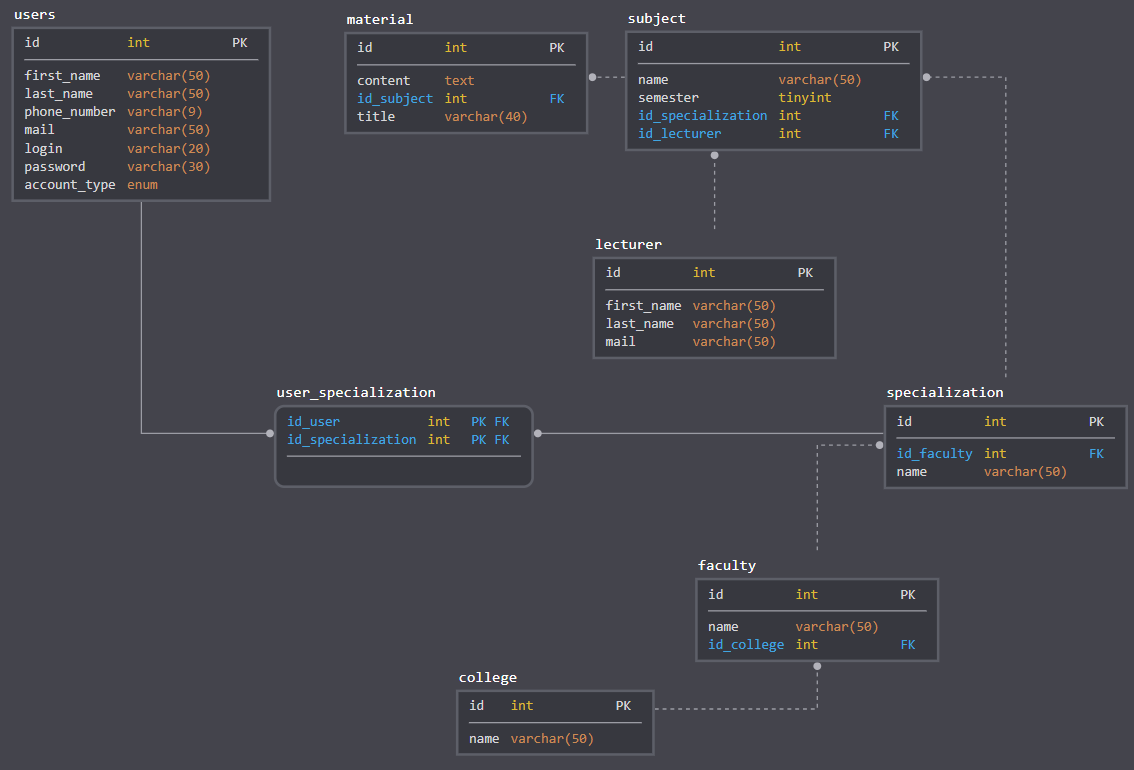
\includegraphics[width=1\linewidth]{relation_model}
			\end{figure}
		\subsection{MySQL}
			Zapytania
		\subsection{Środowisko}
			Baza danych znajduje się w chmurze Heroku. Łączymy się z nią za pomocą...
	\section{Testy}
		Baza działa... Jakieś info z Heroku można tutaj dać.
\end{document}